\chapter{Development and\\Implementation}
\label{cha:implementation}
\chapterquote{It's done, when it's done}{An English Phrase}
The sections in this chapter will describe the various stages of development and implementation of this Bachelor thesis' application. At first the basic idea of the layout and the individual views will be described and explained. To get an even better impression the early paper prototype will be shown. Afterwards a short description of the aspired time schedule for the development as well as the creation of the written elaboration is given.

The implementation of the basic layout which was displayed and explained with the help of the paper prototype, will be the first part describing the actual implementation process.
Second, the handling of the data to be visualized is explained. This covers the server based access as well as local storing and loading. 

After the preparations for the visualization have been set forth, the different views will be described. Starting with the explanation of the map view, it will be clarified how the loaded data is visualized. This is followed by the section focusing on the chart view. It explains how a library is used to draw pie charts and how the loaded data has to be prepared. The last section describes how the timeline was implemented. It covers, how one can draw its own views in Android and how to make use of gestures.
\newpage
\section{Paper Prototype}
\label{sec:paper_prototype}
The first step of the development process was the creation of a paper prototype. It was needed to demonstrate the idea and visual appearance of the project and application. Another advantage of the paper prototype is to be able to show different people the application and get feedback without even writing one line of code. This provides the ability to eliminate possible false estimations  in the forefront of the application's implementation. False estimations may be the assumption of wrong needs of possible future users or the creation of an non intuitive layout. In the following the paper prototype will be shown and explained.

The\mnote{Basic layout} first idea was to split the screen into two parts, an option part and a view part. The left part should be the option part, occupying one sixth of the visible screen. It should always display the following, in appearing order listed, options.\\
In the top left a view selection containing three buttons  ordered vertically with titles ``Map-View'', ``Chart-View'' and ``Timeline'' are displayed. Taping one of those buttons causes a view switch to display the respective view.\\
Under the view selection a list of options should be visible. Those options vary from view to view but should always contain a button at the top of the list displaying the currently selected date. Tapping on this button causes a date-selection-window to pop up. Selecting a date leads to an update of the displayed view, now visualizing the respective data.
Other options will be explained together with their respective views.

When \mnote{Map-View} the application has been loaded, the user will be displayed the map view thus making it the application's start view. The view will display a map with a route, representing the user's visited locations. On start up the selected date will be the current day and therefor the draw route represents the user's latest movements. Tapping on the route should bring up a speech bubble which contains information about the tapped location. Those informations will be the time spend on that location, the used applications and possibly shot photos.\\
The \mnote{Map-View specific options} view provides two special options. The first option is represented by a check box and has the title ``Photos''. The option provides the ability to highlight those locations, where a photo was taken. The second option is called ``Apps''. It lets the user pick applications from a list and colors all parts of the route where those specified applications were used. Those options would provide a great tool to quickly get an overview over the position data of specific applications and actions.

The map view can mainly be used to answer the question ``Where was smartphone used?'', since the view focuses on visualize the map and traveled routes rather than displaying numbers and percentages.
\begin{figure}[h]
	\caption{Map-View}
	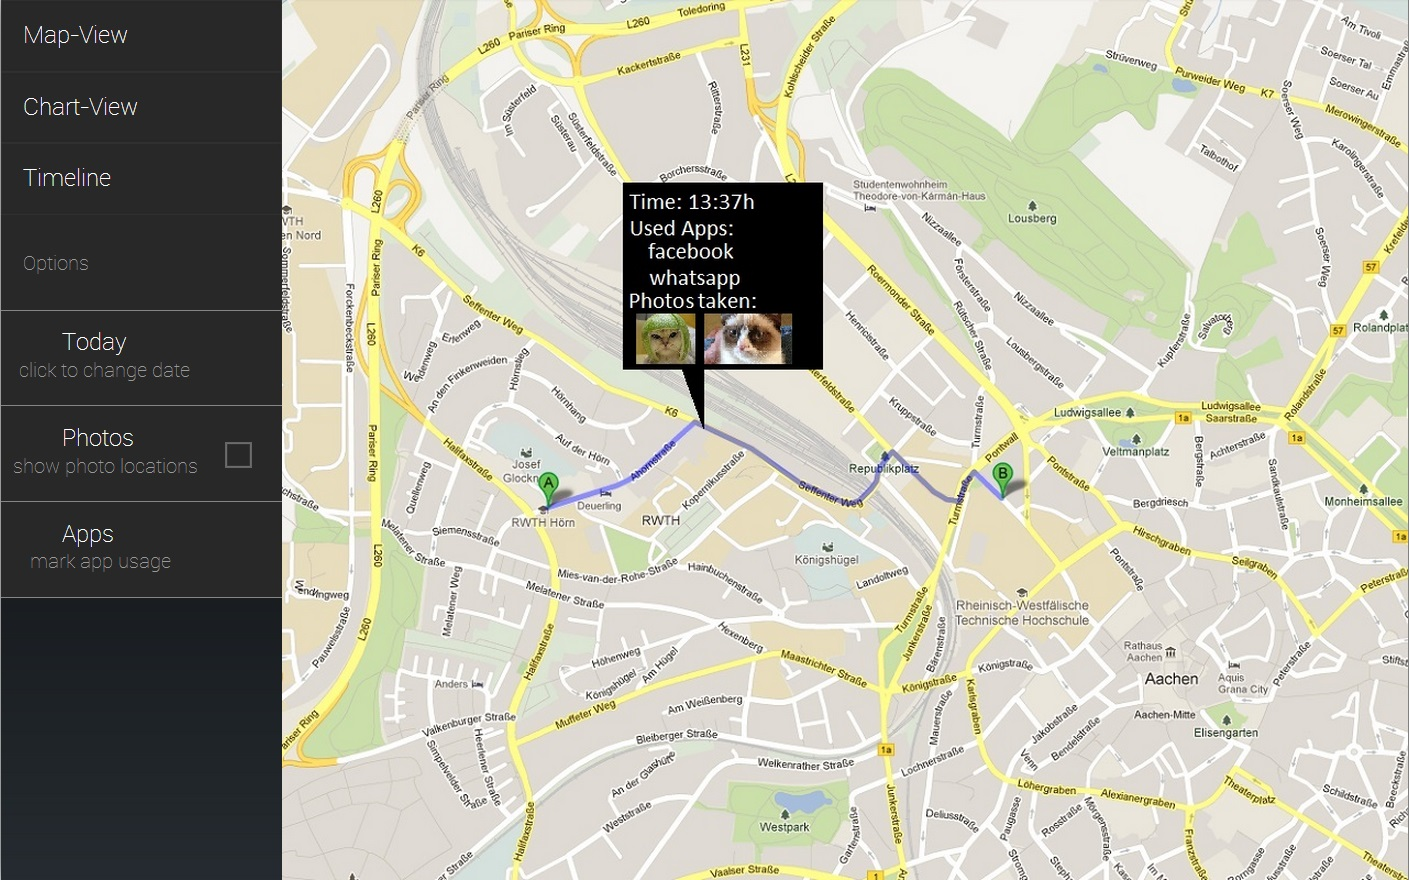
\includegraphics[width=\textwidth]{images/Design/1b_onClickPageView.jpg}
\end{figure}

The \mnote{Chart-View} second view, the chart view, shows the user his or hers daily activities in form of a pie chart. The idea was to create location based charts that shows for each visited place the percentages of used applications. To break down the number of shown charts and thus to give a better overview, locations would be summarized in an intuitive way. That means that one has a chart for work, home and on the move. Those charts are lined up vertically and have an individual chart on the top of the list. This individual chart can be adjusted by the two extra options described in the following.\\
The \mnote{Chart-View specific options} first option lets one choose which places are taken into account for the individual chart. The second option determines which specific applications are displayed in the first chart. With these two options, one has the ability to to customize the first chart to visualize only those data which fit one's individual needs.

To \mnote{Grouping of apps and locations} get an even better overview, applications are classified into different groups. ``Social'' and ``Productive'' could be two groups, which split the applications apart. Applications like whatsapp and facebook may be social, while mail programs would be productive. The user would also be able to classify the applications by him- or herself, allowing to personalize the application. Furthermore, home, work and other places are chosen individually and extra places like parent's home can be added by the user, to give the him or her more space for customization.

To \mnote{Interacting with the view} get an better insight of the application groups, tapping on a slice of the pie chart will bring up a detailed view. In this detail view, one can see which applications are included in the tapped group and how large their percentage of daily activities is. In addition the total usage time of each application is shown, to give the displayed percentages more expressiveness.

The chart view, in contrast to the map view, is able to give a better overview over the percentages of used applications rather than show in which locations they have been utilized. It gives answer to the question ``What was the smartphone used for?''
\begin{figure}[h]
	\caption{Chart-View}
	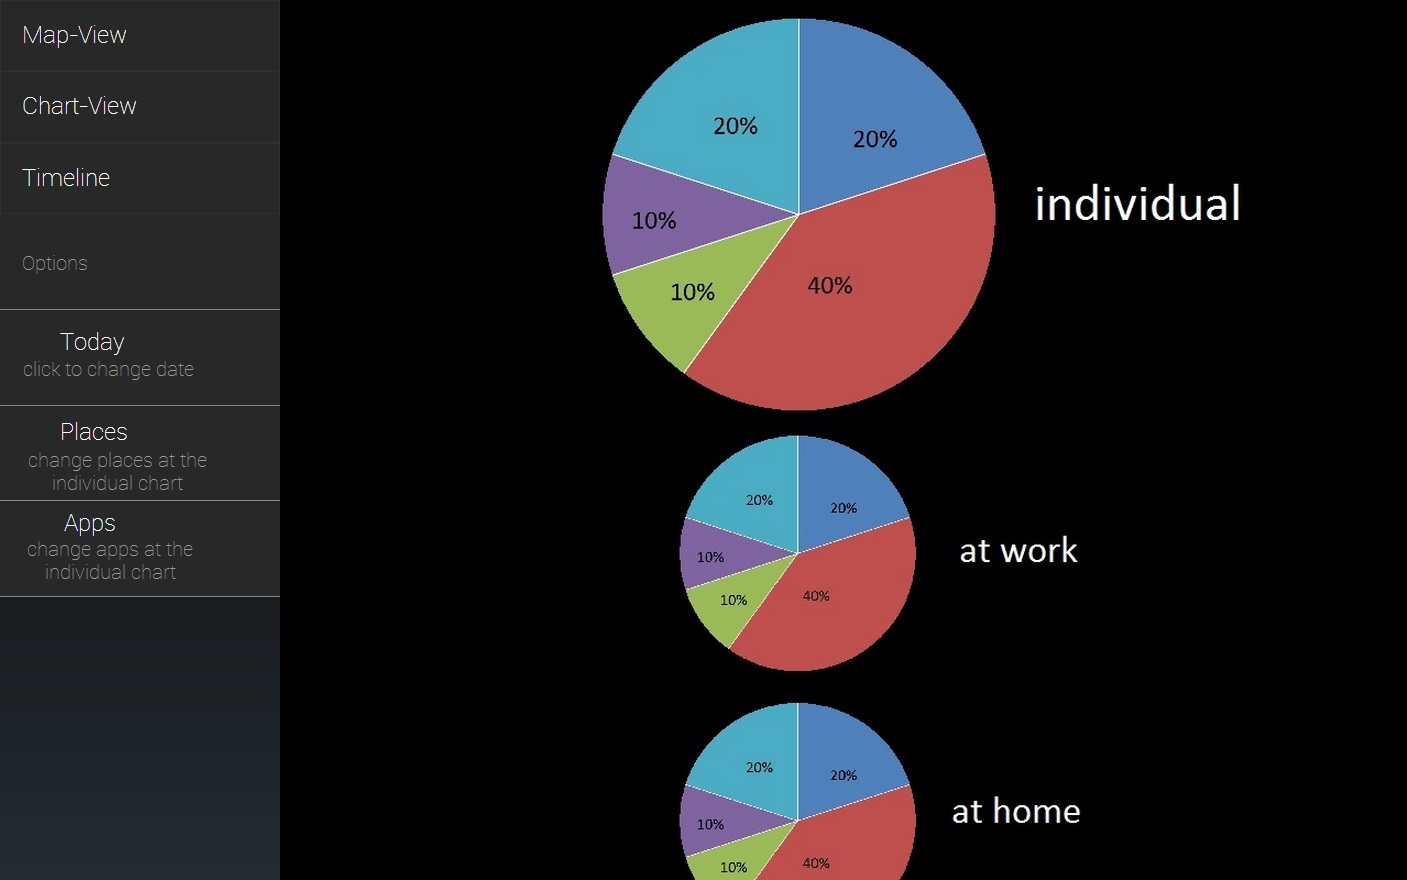
\includegraphics[width=\textwidth]{images/Design/2_ChartView.jpg}
\end{figure}

The \mnote{Timeline} timeline is the third and last view of this thesis' application. This view visualizes the daily activities in a chronological manner with two major parts. The first part is the the timeline itself and is described as follows. At the layout's bottom a horizontal line is draw with markings for every hour, from 0:00 to 24:00. Above this line, colored rectangles are drawn which represent a timespan in which an application was used. At the layout's top one can see markings for the visited location in dependence of the displayed timespan. One has the possibility to scroll horizontally through the view to observe the consecutively occur activities.

Beneath \mnote{The detailed view} the actual timeline a detailed view of all applications used on the selected date is found. This second part shows the application in descending order starting with the application mostly used on the chosen date. For each application a rectangle which represents the percentage of daily usage, is drawn. This rectangle will have the same color as the respective rectangles in the timeline and thus the detailed view can be used as a legend to identify the applications displayed in the timeline. Next to the application's bar the respective percentage and total amount of time is displayed.

This \mnote{Timeline specific options} view offers the extra option ``Apps'', where one can filter the displayed applications. With that option one is able to hide all other applications and display only those which are relevant for the user and thus giving the application a feel of personality and individuality.

Although it partially acts as a bar chart, the timeline, unlike the other views, focuses on the daily schedule by visualize the activities in a chronological order. With this view the user is able to answers the question ``When was the smartphone used?''.
\begin{figure}[h]
	\caption{Timeline}
	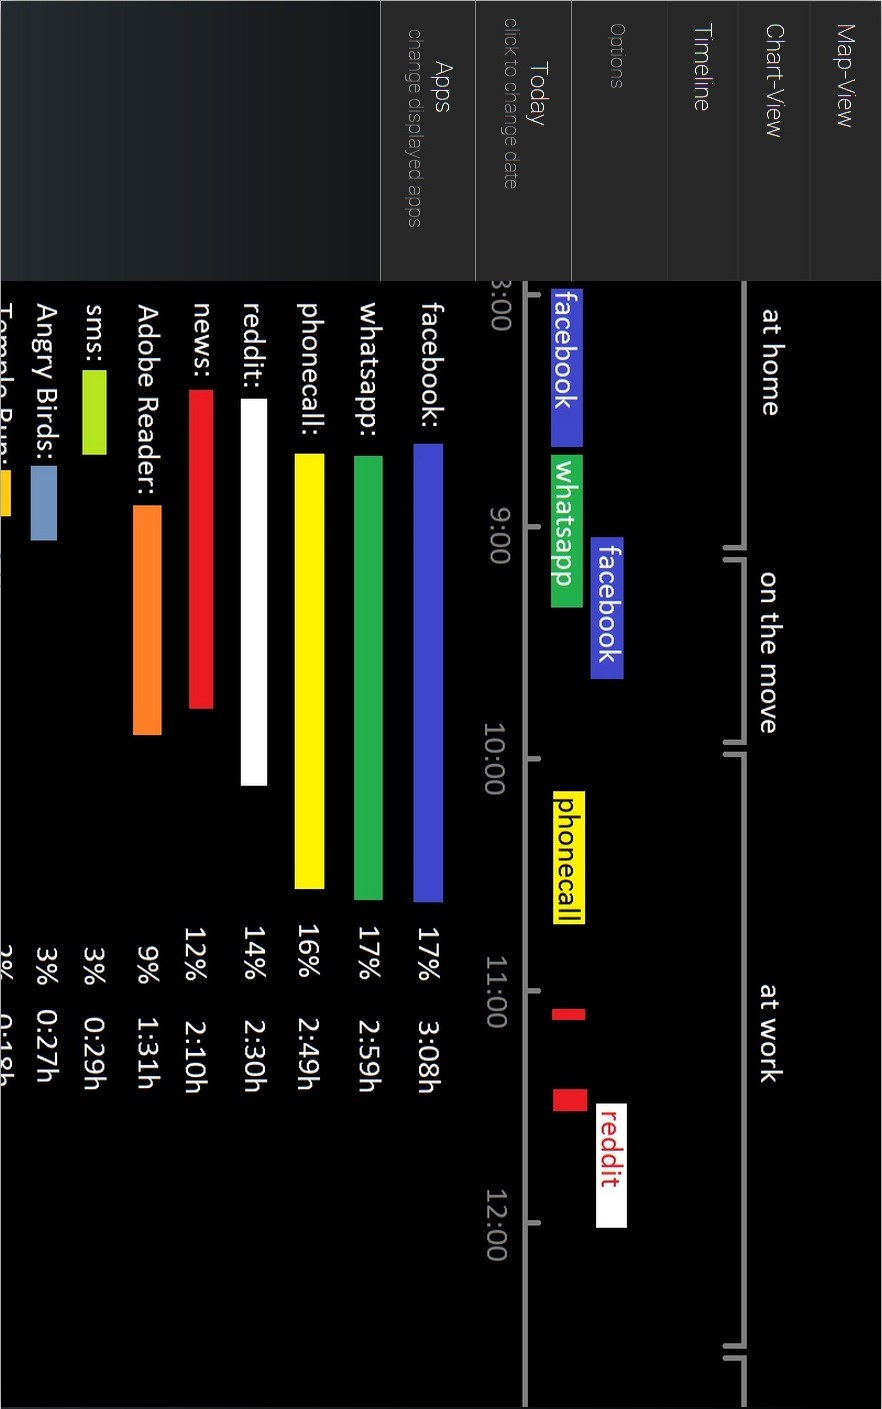
\includegraphics[width=\textwidth]{images/Design/3_TimeLine.jpg}
\end{figure}

As mentioned in the first place, this was the basic idea of the application and a few things have been changed during the development process. A summary of changes which differ from the paper prototype, along with the reasons for those changes can be found in the next sections.

\newpage
\section{Time Schedule}
\label{subsec:time_schedule}

\newpage
\section{Basic Layout}

\newpage
\section{Data Management}

\newpage
\section{Mapview}

\newpage
\section{Chartview}

\newpage
\section{Timeline}

